\section{Theory}
	\subsection{Description of the Geiger-Muller counter}
		The Geiger-Muller (GM) counter works by detecting the ion-electron pairs created by the interaction of charged particles in a gas mixture. The GM tube is a metal cylinder with a thin wire (anode) at its axis and a metal cylinder (cathode) maintained at a high voltage to create an electric field. The radiation enters through a window on the tube, creating ion-electron pairs that are swept by the electric field to produce a phenomenon called an avalanche, which generates output pulses that are counted by related circuits. A schematic diagram of the GM counter is shown in \hyperref[fig:th1]{Figure 1}.

		\begin{figure}[h]
			\centering
			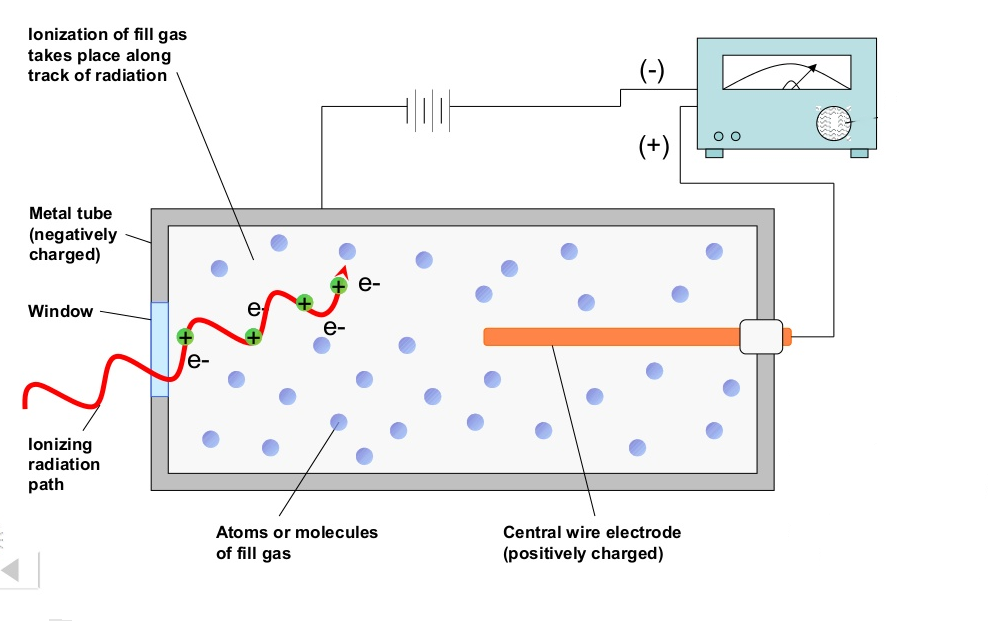
\includegraphics[width=0.8\linewidth]{images/th2.png}
			\caption{Typical GM counter characterstics}
			\label{fig:th1}
		\end{figure}
		
		As shown in \hyperref[fig:th2]{Figure 2} the operating voltage of the GM counter is set in the plateau region, where the counting rate is relatively constant. The plateau length and slope determine the stability of the counting rate, while the dead time, resolving time, and recovery time limit the counting rate. The GM counter is insensitive to ionizing events during the dead time, and the resolving time and recovery time set the minimum time interval between two distinct and normal-size pulses, respectively. Higher voltages and the gas composition inside the GM tube can reduce the effects of these factors. The background counting rate is due to cosmic rays or other active sources in the same room.

		\begin{figure}[h]
			\centering
			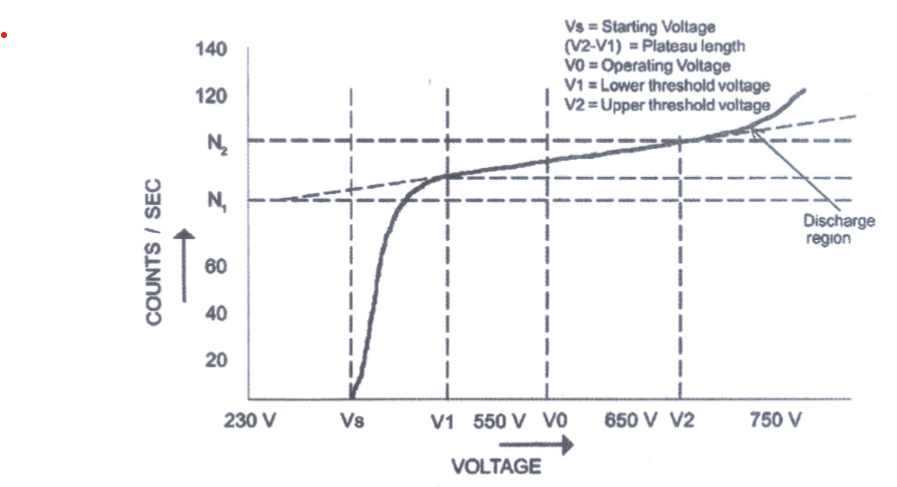
\includegraphics[width=0.8\linewidth]{images/th1.png}
			\caption{Typical GM counter characterstics}
			\label{fig:th2}
		\end{figure}
	
	\subsection{Inverse square law: Gamma rays}

		It states that the gamma radiations reduce inversely proportional to the distance, D, between the detector and the radiation source. Thus, the counting rate, R (counts/second), should be related as follows:

		$$R \propto \frac{1}{D^2}$$

		$$\therefore\log(R) = -2\times\log(D) + c$$

		where c is some constant

	\subsection{Efficiency of GM counter}

		Knowing the activity of that specific source allows one to calculate the effectiveness of a GM counter. The quantity of the radiation source's disintegrations per second is known as activity. The ratio of the observed counts per second to the number of disintegrations that are detected by the detector each second is referred to as the efficiency. The efficiency, E, is now:

		\begin{equation}
			E = \frac{CPS}{DPS}\times100
			\label{eq:1}
		\end{equation}

		where CPS is the counts per second, and DPS is the disintegrations per second, falling on the window of the detector. DPS can be calculated as:

		\begin{equation}
			DPS = A\frac{d^2}{16D^2}
			\label{eq:2}
		\end{equation}

		where A is the activity of the source, d is the diameter of the detector, and D is the distance between the source and the detector.

	\subsection{Counting Statistics}

		Say $N_i$ denote the $i^{th}$ reading of a measurement in a set of $n$ measurements, then the equations for calculating mean ($\bar{N}$), variance $\sigma^2$, and standard deviation $\sigma$ (for large samples) are:

		$$\bar{N} = \frac{1}{N}\sum_{i = 1}^{n} N_i$$

		$$\sigma^2 = \frac{1}{n} \sum_{i = 1}^{n} (\bar{N} - N_i)$$

